\chapter{Aim of the Work}

The metamorphic self-reconfigurable robots have several properties which makes
them an appealing direction for future robotics trends. Let us remind some
of these properties:
\begin{itemize}
    \item The uniform modules should become cheap and fast to mass-produce just
    like we have seen in the case of a production of integrated circuits in the
    recent decades.
    \item The reconfigurability of such robots should make them versatile and
    easy to adapt for particular application.
    \item The self-reconfiguration property of the robots could bring us closer
    to rapid prototyping of robots. We could treat robots just like we treat
    software -- the developers just write some kind of descriptions and by
    running a \texttt{make} command, the robots self-assembles. Such ability
    would also allow us to easily version-control robots with an easy option to
    roll-back to an older revision without the necessity of keeping a physical
    inventory of older version.
    \item On top of that, such robots can be highly fault tolerant. If designed
    suitably, there is no single point of failure (e.g., in a form a single
    actuator or control unit). Also, such robots could repair autonomously
    compared to traditional robotics.
\end{itemize}

However, in the current state of the art we are far away from reaching these
properties in practice. As we showed in Chapter \ref{chap:state-of-the-art}, the
research in this area is broad and vivid. Yet, there are plenty of challenges
and open-problems to tackle.

From all the challenges that metamorphic robots present, I would like to focus
on finding ways to control metamorphic robots in fault-tolerant manner via
distributed control in my research. I further describe my goals in the following
text.

\section{Controlling Metamorphic Robots}

There are several point of view on different level of abstraction on the control
of metamorphic robots. Basically, we can separate it into two classes of
control: reconfiguration and locomotion.

Reconfiguration presents the problem of moving individual modules in the system
to change the system's shape. Usually the proposed solution operate on top of
simple motions primitives (e.g., move joint, connect or disconnect) and expect
that the system has a way of synchronous execution of these primitives. The
output is a schedule of the motions primitives. When such schedule is
executed, the shape of the system is changed. \todo{Cite reconfiguration papers}

Locomotion of metamorphic robots deals with the problem of transporting the
robotic system in space so it can interact with the outer world. The solution
for the locomotion comes in the form a controller for prescribed configuration
(e.g., as in the case of \todo{cite}). The locomotion problem often involves
inter module synchronization and communication.

There is also a combination of both approaches; e.g., locomotion via
reconfiguration or a locomotion controller which uses reconfiguration as a
procedure to change system's shape when needed.

In my research I would like omit the reconfiguration part from the control and
mainly focused on designing controllers that perform given task without changing
the robot shape.

\section{Concept of Fault-tolerance for Metamorphic Robots}

\todo{Move to intruduction? Preliminaries? State of the art?}

There is no single widely accepted interpretation of what fault tolerant systems
should comply to. Usually, in a context of embedded system, a system is
considered fault-tolerant when it is able to continue operating (possibly with
worse performance) after one of its components fails
\cite{DBLP:journals/micro/Johnson84}. The extent of fault-tolerance depends on
what type of failures the system survives.

For example, we usually consider living organisms as highly fault-tolerant
systems. If an animal looses an limb, it is able to adapt and perform similar
tasks. E.g., a cat without a leg is still able to move and climb -- possibly
slower, but it is able to survive.

In the context of metamorphic robots, \textcite{DKbotDistr} discuss several
aspects of fault-tolerance and for some of them they propose solutions. They
distinguish several types of fault:

\paragraph{Complete module malfunction,} where the module stops responding and
acts passively. The usual assumption is that the other modules in the system can
detect such module. This type of malfunction is probably the most mentioned one
in the literature. The usual solution is to either drop or to ignore such
modules and reconfigure into a new configuration
\cite{DBLP:conf/ieeealife/Christensen07, DMotionCoord}.

\paragraph{Byzantine module malfunction,} where it is not easy to detect the
module has failed -- e.g., the module can have a wrong sensor and it can report
wrong data to other modules. The module can even be malicious. There is not much
work on this type of malfunction in the context of metamorphic robots as far as
we aware. However, in context of distributed systems in general, it is a vivid
research topic. E.g., work by \textcite{DBLP:conf/osdi/CastroL99} could be
adapted for metamorphic robots.

\paragraph{Actuator malfunction,} where the module control unit is fully
functional, however, one or more of the modules actuators are either stuck
in a position or spin freely. This type of malfunction was tackled by
\textcite{DBLP:conf/romoco/VonasekONW15}.

\paragraph{Explosion of the whole system} is a type of malfunction where the
robot is broken down into pieces randomly spattered over the environment usually
after a high energy impact. \textcite{DBLP:conf/iros/YimSSPDT07a} proposed a
solution for automatic reassembly after explosion. They also discuss, that
system explosion is a way of fault-avoidance. When a system can reassemble, it
is desirable to include weak, re-attachable joints, which protect the individual
modules.

In my research, I would like to focus on a partial module malfunction, since
system explosion is more related to research about spatial localization and path
planning than distributed control. Similarly, complete module malfunction is
probably better solved by reconfiguration as distributed control has no other
option to deal with a completely malfunctioned module than to ignore it.

A robot without sensors cannot interact with the environment and can only follow
hard-coded paths and therefore, can be used only a highly controlled
environment. This is contrary to the overall motivation for metamorphic robots,
therefore these robots have to feature a large number of sensor. In practice,
one can expect that some of this sensors can report faulty readings or become
faulty. Similarly, with large number of communicating nodes, we can expect
communication errors to be present. Therefore, I would like more specifically
propose a solution for controlling metamorphic systems where the individual
modules can feature Byzantine faults originating from their sensors or faulty
communication.

\section{Distributed Control}

\todo{I would like to somehow state that most of the solutions out there are centralized and not actually executed on the robots. But how should I do that?}

\section{Proposed Case Studies}

During my PhD study I would like to perform two case studies to tackle the
challenges I stated above. That is to design a distributed controllers for
specific configurations, which allow the system to transport in space and be
fault tolerant for partial module failures. After performing those case
studies, I would like to generalize the findings and to introduce a more general
approaches if applicable.

\begin{figure}[!t]
    \centering
    \begin{subfigure}[b]{0.45\textwidth}
        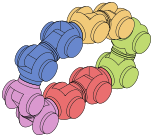
\includegraphics[width=\textwidth]{figures/ring_example.pdf}
        \caption{Loop Robot}
        \label{fig:example_roller}
    \end{subfigure}
    ~
    \begin{subfigure}[b]{0.45\textwidth}
        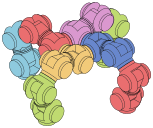
\includegraphics[width=\textwidth]{figures/spider_example.pdf}
        \caption{Walker Robot}
        \label{fig:example_spider}
    \end{subfigure}

    \caption{Examples of metamorphic systems for the case studies.}
\end{figure}

\subsection{Loop Robot}

In the first case study, I would like extend or redesign the controller
developed by \textcite{DBLP:journals/ijrr/SastraCY09}. In their work, they
designed a centralized controlled for a simple ring robot formed out of variable
number of modules (see Figure \ref{fig:example_roller} for an example of such
system). The robot can move forward by rolling. This paper leverages the
dynamics of the system to move faster compared to previous work. The controller
uses accelerometers in the modules as feedback.

I plan to introduce the following improvements:
\begin{itemize}
    \item I will transform the controller into a distributed one as the first
    step towards fault tolerance. This presents mainly a challenge in
    synchronization and information exchange.
    \item Then I would like to remove the assumption, that the individual
    modules report correct feedback. The controller should be able to deal with
    some number of units that provide incorrect feedback.
    \item If applicable, the controller should also be able to deal with some
    number of units that have faulty joints.
\end{itemize}

\subsection{Walker Robot}

In the second case study, I would like to dive deeper into the problem of
performing synchronized actions (especially movements) and more specifically,
focus on removing the bottle-neck of distributed controllers -- the bottle-neck
in form of the limited speed and bandwidth of communication lines between the
modules. There were proposed solutions for synchronization in such systems, but
they do not scale well with increased number of modules in the system.

Therefore, as a first step in this case study, I would like to take a
non-trivial configuration (e.g., walker in Figure \ref{fig:example_spider}) and
designed a mechanism for synchronous execution of a movement (prescribed by a
gait table) which scales well with the number modules. The scalability should be
achieved by dividing the system into a hierarchical cluster. Cluster members
should be able to synchronize with each other and the cluster should synchronize
among themselves. I would like to leverage findings about communication fault
tolerance from the loop robot case study and apply them to this environment as
well. Possibly, this work could be seen as extension of the concept of robotic
hormones introduced by \textcite{DBLP:conf/icra/SalemiSW01} and further extended
in \cite{DBLP:journals/trob/ShenSW02}.

The second step of this case study should be replacement of the gait tables by
individual controllers which not only require synchronization, but also require
inter-cluster feedback. I expect this part of the case study to be
generalizable.

\section{Evaluation Platform}

I would like to demonstrate the proposed solutions on a physical robots. I would
also like to make my research as reproducible as possible. That is unfortunately
quite hard in the area of robotics as one cannot easily download a robot and
test my solutions.

To achieve the best reproducibility as possible, it is crucial to use a hardware
platform which is easily obtainable. In the section \todo{Ref to existing
platforms} we provided a list of existing platforms for modular, self
reconfigurable robots. None of the platforms has manufacturing data (for
mechanical construction and PCBs) nor firmware publicly available. We also
contacted the authors if they are willing to share their design files or if
there is a possibility to buy their robots. Unfortunately none of them responded
positively. Only the authors of SMORES (\todo{citace}) responded that it would
be possible to cooperate and try our solutions on their robots at their
facility, which is not convenient.

Therefore, I set an additional goals of my PhD study: I would like to develop an
open-hardware and open-source platform for metamorphic distributed robots. This
platform should serve as tool for demonstration of my research outcomes which
allows the others to easily build their own robots and reproduce my results.
Also, by being the first open platform, it should serve as a research tool for
the others in the area.

The platform, called the RoFI platform, is part of my study I have advanced the
most so far and we introduce more in detail in Chapter \ref{chap:results}.

\section{Time Plan}

\todo{Let's make the schedule}
